% Relay — main file. Compile: tectonic relay.tex (or make -C . pdf)
% Template: house conventions (obviousbench + answer-key papers) via benchkit.
% Body lives in sections/*.tex; tables under tables/ are GENERATED
% (relay_analysis.py, relay_gates.py) — do not hand-edit either.
\documentclass[11pt]{article}
\usepackage[margin=1.05in]{geometry}
\usepackage[T1]{fontenc}
\usepackage{newtxtext,newtxmath}
\usepackage{booktabs}
\usepackage{graphicx}
\usepackage{microtype}
\usepackage{tabularx}
\usepackage[numbers,sort&compress]{natbib}
\usepackage[hidelinks]{hyperref}
\usepackage{xcolor}
\usepackage[section]{placeins}
\usepackage{flafter}
\usepackage{fewerfloatpages}
\usepackage{fontspec}
\newfontfamily\iconfont{FreeSerif.otf}
\newcommand{\lunaicon}{{\iconfont ☾}}
\newcommand{\terraicon}{{\iconfont ⊕}}
\newcommand{\solicon}{{\iconfont ☼}}

% House style from the kit: captions (tables captioned above), \Cref
% cross-references, compact references, float placement, table notes.
\usepackage[housestyle]{benchkit}% vendored by benchkit sync (see .benchkit.json); load after hyperref and natbib
\newcommand{\blindboard}{\benchmarkname{Blindboard}}
\newcommand{\relay}{\benchmarkname{Blindboard Relay}}
\newcommand{\snapshotname}{relay-2026-09}
\benchkitsnapshot{tables/relay_macros}% generated census/cost/floor macros — numbers never hand-typed

\title{Blindboard Relay: Measuring Model-Written Memory\\
Across Amnesiac Turns}
\author{Adam Allcock\\
Independent researcher\\
\texttt{adamallcock@gmail.com}}
\date{Preprint, October 2026}

\begin{document}
\maketitle

\begin{abstract}
\relay{} tests whether language models can write notes that a fresh instance can use on the next turn. In \blindboard{}, a hidden-keyboard deduction game, each turn receives the fixed rules, one predecessor note and the current observation. The client discards the earlier transcript and reasoning. The score is the fraction of keys identified correctly. A sound reference policy supplies an attainable score at each note budget. We sample combinations of nine models from three providers, seven budgets and four text interfaces, with visible-transcript and retained-reasoning controls. At 100 characters, GPT-5.4 Nano's notes score $\relayfamsevenabs$ below its retained-reasoning control ($p\relayfamsevenp$); these conditions were collected on different dates. A supplied schema improves Nano's notes by $\relayprimnanoschematwohundreddelta$ at 200 characters and $\relayprimnanoschemafiftydelta$ at 50, surviving correction over the declared \relayprimfamily-test family. Schema notes also outperform Nano's visible transcript, but the later retained-reasoning control scores $\relayfamfivestdabs$ higher than the schema. Same-day tests on fresh seeds confirm higher scores with retained reasoning for GPT-5.6 Luna and GPT-6 Luna. GPT-6 Sol, Gemini 3.8 Flash and Claude Opus 5.5 score at least $\relayfrontiermin$ in every tested condition at 100 characters. Tighter budgets lower their scores but do not establish a ranking. Adjacent note formats become more similar within longer chains, but the metric does not establish chain-specific conventions. These pilot results, at one reasoning effort, support model-specific memory tests. Frontier rankings and transfer to open-world agent memory remain unestablished.
\end{abstract}

\clearpage
\section{Introduction}

Language-model agents often store summaries, scratchpads and handoff notes for later calls. A retained transcript can make it hard to tell how well a model selects and encodes the information a later call needs.

\relay{} studies this question in \blindboard{} \citep{blindboard2026}, a hidden-keyboard deduction game. The model presses a chord, or group of keys, and receives their symbols as an unordered set. Announced rotations move symbols between keys. The final score is the fraction of keys identified correctly. Each relay turn starts a new request with the rules, the current observation and one note written by the preceding call. Earlier messages and reasoning are discarded.

We vary the note interface: free-form text, a supplied schema, a self-designed notation specification repeated on every turn, or a structured form serialized by the experiment software (the harness). Each has a hard note budget. An exploratory image condition carries a rendered Scalable Vector Graphics (SVG) image instead of text. These conditions compare complete interface packages: they differ in assistance as well as notation. The rules and observation do not count toward the note budget.

\Cref{fig:loop} follows three turns of a stored episode. Each fresh instance reads its predecessor's note, presses four keys and writes a note for its successor. The note must preserve any information the next instance needs beyond what its observation supplies. We compare note conditions with two transcript controls (\Cref{fig:loop}, bottom). The visible-transcript control resends every earlier observation and reply; the retained-reasoning control also replays the model's earlier reasoning.

\begin{figure}[t]
\centering
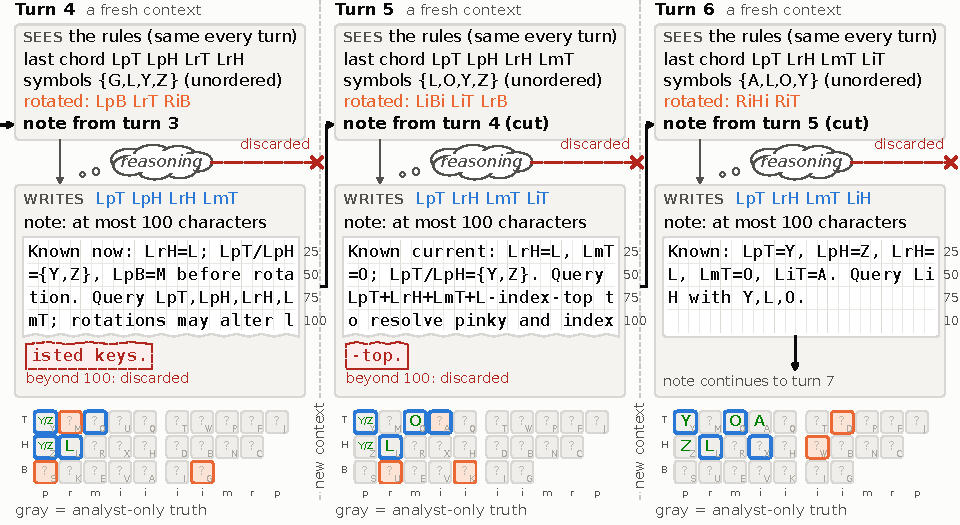
\includegraphics[width=\linewidth]{figures/relay_figA_loop.pdf}\\[5pt]
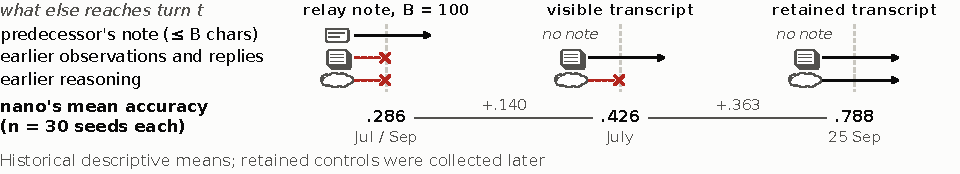
\includegraphics[width=\linewidth]{figures/relay_figA_regimes.pdf}
\caption{Inputs and notes across relay turns, with transcript controls for comparison. Top: turns 4--6 of one stored GPT-5.6 Luna episode (free-form notes, $B{=}100$ characters, seed 0). Each fresh instance receives the rules, the current observation and one note; earlier transcript and reasoning are discarded. Chords return unordered symbol sets. Key names follow the model's notation (LpT: left pinky, top row). Green shows what the note states, blue outlines the keys pressed, and orange marks keys named in the rotation notice. Small gray letters show the hidden layout as analyst annotations; the model never sees them. Cards show outgoing, not incoming, notes. Bottom: the three interfaces and GPT-5.4 Nano's historical mean board accuracy (fraction of keys correct; $n{=}30$ seeds per condition). The retained control was collected later (\Cref{tab:ladder}).}
\label{fig:loop}
\end{figure}

The conditions share game rules, reference calibrations, diagnostics, seeds and baselines. Small contexts keep episode costs to cents. Most reported cells contain $n{=}10$ seed-paired episodes; some contain 15, 20 or 30, and two Sol cells contain 5. \Cref{app:cells} gives the exact $n$ for every reported text-channel cell, separated by prompt version.

\paragraph{Contributions.}
\begin{enumerate}
\item \textbf{A relay protocol}: fresh model instances pass one authored note under a hard budget. The harness rebuilds the context each turn, replays no earlier transcript or reasoning, and stores notes verbatim.
\item \textbf{A budget-matched reference}: a sound solver uses the same channel with a truncation-aware encoder and decoder (codec). Deterministic calibrations measure what this specified policy can achieve at each budget. Both codec generations are archived (\Cref{sec:reference}).
\item \textbf{A scaffolding comparison}: paired-seed tests compare free-form notes, an imposed schema, a pinned self-designed notation specification (the constitution condition), and a harness-validated form. Visible-transcript and retained-reasoning controls provide separate comparators.
\item \textbf{Behavioral evidence}: a stored corpus of \relaystorednotes{} notes, including legacy and coaching-audit records; a note-format drift measure with a fixed-codec negative control; and a pixel channel with a separate fidelity probe. The main v2 text runs contain 15,930 notes, including 573 terminal outputs that no successor receives. Legacy and coaching-audit runs contain 1,792 and 779 notes, respectively. Four newer models from three providers test which findings extend beyond the original roster (\Cref{sec:added}).
\end{enumerate}

The base environment is public \citep{blindboarddata2026}. The per-model memory-tool screen costs about \$\relayfitcostnano--\$\relayfitcostsol{} before deployment (\Cref{sec:discussion}).

\subsection{Related work}\label{sec:related}

Agent-memory benchmarks test recall within a persistent context or memory store: long conversations \citep{locomo2024}, enterprise timelines \citep{memtrack2025}, dynamic environments \citep{gaia226,evoarena2026}, and multi-session applications \citep{memoryarena2026,memgym2026}. Staleness tests ask whether old facts still hold \citep{stale2026}. \relay{} resets the model every turn and measures performance with the note that survives. Architectural comparisons in signaling games \citep{signals2026} show that memory interfaces matter, but do not require hidden-state deduction or certify what fits in a fixed channel.

Other work directly evaluates budgeted memory writing. \citet{memaudit2026} score memory selection against an exact optimum for a fixed candidate package, separating writing from downstream retrieval and reading. \citet{budgetbench2026} vary the total active-context allowance when comparing memory strategies. In a signaling game, \citet{signals2026} use an overwritten 150-word scratchpad and fixed-capacity codebooks alongside a rolling 20-round history. Relay combines repeated, self-authored replacement notes with hidden-state deduction and a hard code-point budget. It also supplies a versioned sound reference policy and separate visible-transcript and retained-reasoning controls. The measured unit is the complete interface package, not writing alone or optimal channel capacity.

Compression methods shorten supplied content \citep{llmlingua2023,gist2023,autocompressors2023,icae2023,raptor2024}. Self-managed memory systems let an agent curate a persistent store \citep{memgpt2023,generativeagents2023,latentctx2026}; budgeted consolidation determines which records remain in that store \citep{retainconsolidate2026}. In Relay, a note is written from one turn's context and replaces its predecessor completely. The writer must choose the facts, their encoding and any plan the next instance needs. A rate-distortion account of agent memory \citep{ratedistortion2026} motivates the trade-off between memory size and decision-relevant information. Our sound reference supplies an attainable score, or floor, for this game.

Transmission-chain experiments pass artifacts between generations \citep{kirby2001,kirby2008,acerbi2023}. The closest advice-based task uses fresh learners and written advice \citep{colas2025}. Relay adds a hard character budget and checkable state within one episode, while keeping model weights fixed. Self-notes and reflection also produce written artifacts \citep{selfnotes2023,reflexion2023,expel2023}, and chain-of-agents pipelines relay summaries \citep{chainofagents2024}. These approaches do not combine total context resets with a budget-matched reference. Our pixel channel tests a model's own visual memory encoding, rather than only its reading of supplied visual text \citep{vistabench2026,visionwormhole2026}. \Cref{app:related} gives detailed comparisons, including latent-state relay compression.

\section{Benchmark and measurement}

\subsection{Base game}
An episode follows \blindboard{} \citep{blindboard2026}. The $N$ keys have a hidden one-to-one mapping to symbols. The model presses chords of $K$ distinct keys, addressed by touch-typing coordinates, and receives their symbols as unordered sets. Between turns, announced rotations move symbols among subsets of keys. Each rotation is a derangement: every selected key changes symbol. The model may end the game with a full-board guess on any turn and must guess after at most $T$ press turns. Board accuracy is the fraction of keys correct in the layout at the time of the guess. Optional locks have a separate score and do not freeze the layout.

The relay base has 26 keys, $K{=}4$, a 20-turn cap and rotations ending by turn 9. The full-memory reference solves the evaluated instances, and every interface uses the same world rules. A 39-key base supports the transfer experiment; a 60-turn-cap base supports the drift experiment and frontier test F17. Caps do not require models to complete that many turns.

\subsection{The relay loop}\label{sec:loop}
Each turn receives the system rules, the predecessor's note, the current observation and a wrapper reporting whether the note exceeded its budget. The constitution condition also repeats its pre-game notation specification. The context starts with two fresh messages and server-side storage disabled; no earlier transcript or reasoning is replayed.

The observation gives the turn and phase, previous ordered presses and unordered results, rotation notices, and environment feedback. Re-locking a key produces an ``already locked'' notice. This does not reveal whether the lock was correct, but it can reveal an earlier action outside the note budget. The note is therefore the only budgeted authored memory, not the only possible source of information about the past. Only a same-turn correction retry can extend the turn's context (\relayretrycalls{} calls across main-v2 text-note episodes). A retry replays the rejected reply's text, but not its reasoning.

The v2 rules state that notes do not accumulate and that the successor's observation echoes the current turn's presses and results. They also retain two coaching sentences: invent a dense, consistent notation; and record layout knowledge, uncertainty and plans. These instructions concern behavior the benchmark measures, so we treat them as part of the instrument. We tested a controlled \texttt{nocoach} variant with both sentences removed on each of the four original models (\Cref{sec:audit}). \Cref{app:prompts} reproduces the relay-mode rules and imposed-schema notation verbatim. The remaining condition blocks (form, image and constitution pin) will be included in the publication artifact, \texttt{relay/prompts.py}.

\subsection{Channels and conditions}\label{sec:channels}
\textbf{Text budgets.} The budgets are $B \in \{800, 200, 100, 75, 50, 30, 25\}$ Unicode code points, the units counted as characters here. The harness carries only the first $B$ code points. This can split a word, token or grapheme cluster (a user-perceived character) and does not fix the number of bytes or bits. The cut is announced as ``torn off.'' The budget excludes shared rules, action echoes, feedback, overflow markers and condition-specific instructions. Ordered press echoes and overflow markers can carry additional information; we did not measure their use as communication channels.

The budget range was not fixed in advance. The pilot grid was $\{800, 200, 100, 50, 25\}$. We added $B{=}75$ after the pilot located the mid-tier retention crossing (\Cref{sec:reference}). We added $B{=}30$ after GPT-5.6 Sol produced a positional encoding at $B{=}50$. A budget above 26--27 leaves room for one character per key without explicitly suggesting that encoding. Both budget choices were exploratory. Later families at an already chosen budget were declared before their own collection; they test that condition, not the budget-selection process (\Cref{sec:setup}).

\textbf{Schema.} The rules specify and require our codec: key indices, \texttt{!} for singleton facts, and \texttt{|} for set facts.

\textbf{Constitution.} One pre-game call designs a $\leq$400-character notation specification. The harness then pins it verbatim in every turn's system prompt, outside the note budget.

\textbf{Form.} The action JSON (JavaScript Object Notation) includes structured \texttt{known}/\texttt{groups} fields. The harness checks addresses, symbols and entry shapes, dropping and counting invalid entries. It does not verify factual truth or all one-to-one mapping constraints. It renders the accepted entries in a fixed mnemonic format and passes that rendering as the note. The protocol thus enforces the notation.

\textbf{SVG} (Scalable Vector Graphics). The model returns SVG source ($\leq$2{,}500 bytes), filtered for script, image and resource-reference patterns. For this snapshot, macOS Quick Look (\texttt{qlmanage}, macOS 26.5.2) rasterized each SVG at 512px. The successor receives only the rendered PNG (Portable Network Graphics) image. The stored images are the channel record.

The \textbf{transcription probe} tests recovery from a simpler state than the game. One instance encodes a supplied random 10-fact state as SVG; a fresh instance reads the rendered image back. Recovery precision and recall measure the combined write$\to$render$\to$read process. They do not identify the source of game failures.

\subsection{The budget-matched reference}\label{sec:reference}

The reference codec writes deduced singleton facts first, at 2 characters per fact, followed by set constraints. When shorter, it uses a positional string: one character per key, with \texttt{?} for unknowns. We adopted this encoding from GPT-5.6 Sol (\Cref{sec:b30}). Truncation retains only complete entries. Decoding a truncated serialization of a sound tracker preserves soundness: retained deductions remain valid. Property tests check this at every possible cut point. The decoder skips some malformed entries, but can accept correctly formatted false facts, and contradictory entries can raise an error. The guarantee covers truncation, not arbitrary corruption.

The reference cuts at entry boundaries. Model notes are sliced after $B$ Unicode code points, potentially within a word or encoded fact. This deliberate asymmetry measures what a sound, truncation-aware encoder achieves. Models may adopt the same property, as Sol does.

Each turn, the reference reconstructs its belief tracker and lock set from the note; its seeded random-number generator persists. Its score curve depends on this policy-state convention and the free observation. The reference is \textbf{deterministic}: layout sampling and chord scoring do not depend on the interpreter's hash seed. Certification is stored as a local, versioned artifact that can be reproduced exactly: \texttt{calibration-codecv2.json}. It contains per-seed floors for 40 seeds, which a release gate re-derives seed by seed at the contested budgets.

Across these 40 relay-base trajectories, the shortest full-state serialization under this policy peaks at \textbf{65 characters}. The note-based reference scores $1.000$ at every $B \geq 50$, $\relayfloorbthirty$ at $B{=}30$ (standard error $.013$), and $.459$ at $B{=}25$. The 65-character peak is a maximum over this policy's evaluated trajectories, not a bound over all sound states or policies. We also retain the earlier entry-only codec calibration, \texttt{calibration-codecv1.json}. Adding the positional encoding raised the $B{=}50$ floor from $.946$ to $1.000$ and left the $B{=}30$/$25$ floors unchanged. Thus, full solvability at budgets $\geq 50$ is a codec-v2 result, whereas the observed $B{=}30$ floor is unchanged between these two codecs.

On the 39-key transfer base, the same policy's shortest full-state serialization peaks at 97 characters across 40 evaluated trajectories. It achieves a floor of $1.000$ at $B \geq 100$. The calibration is retained as \texttt{calibration-codecv2-numrow.json} and re-derived by the same gate. The policy solves all 40 relay-base instances at $B \geq 50$; the note budget therefore permits a solution on each. Model failures may still arise from chord selection, deduction, notation or stopping policy; calibration does not isolate these causes.

For descriptive summaries, we define the \textbf{operational 80\%-retention crossing} as the smallest observed budget whose cell mean reaches 80\% of the model's visible-transcript mean (\Cref{sec:setup}). This is a threshold convention, not an estimated changepoint. Under a 75\% rule, Sol's crossing moves to $B{=}\relaycrossingseventyfivesol$, while Luna's stays at $B{=}\relaycrossingseventyfiveluna$. The model-to-reference crossing ratio is descriptive. The reference crosses at $B{=}50$, where its score is $1.000$.

\subsection{Experimental setup}\label{sec:setup}

The original models are GPT-5.4 Nano and GPT-5.6 Luna, Terra and Sol, referred to below as Nano, Luna, Terra and Sol. They use medium reasoning effort. Four added models are GPT-6 Luna, GPT-6 Sol, Gemini 3.8 Flash and Claude Opus 5.5 (Opus 5.5). Gemini 3.5 Flash supplies a separate replication. Each model has one fixed effort setting; model and effort must be interpreted together \citep{blindboard2026}.

The corpus contains \relaystoredepisodes{} stored episodes: \relayprintedepisodes{} main text-channel episodes, 25 pixel-channel episodes, \relayrefusedepisodes{} excluded pilot episodes and 40 prompt-audit episodes. It also contains \relayprobepairs{} transcription-probe pairs. Most cells use seeds 0--9; \Cref{app:cells} gives every cell's count and prompt version. An illegal action receives one corrective retry; another illegal action forfeits the turn. Forfeiture affected \relayforfeitepisodes{} of the reported episodes.

Recorded cost is approximately \$\relaycostlist{} at collection-date list prices, including cached-input rates where usage is itemized. This includes 40 constitution-design calls, whose usage is recovered from episode totals minus itemized game calls. About \$2 in additional probe calls is unitemized; the refused Sol attempt has no stored itemized cost. These are recorded list-price equivalents, not a complete invoice reconciliation. OpenAI ran on flex; Opus 5.5 and Gemini 3.8 Flash ran on standard tiers.

\paragraph{Transcript controls.}
Both controls replay the rules, every observation and every earlier reply without truncation. The \emph{visible-transcript control} discards earlier reasoning. The \emph{retained-reasoning control} replays all earlier output items through the provider's native mechanism: encrypted reasoning items for OpenAI, signed thinking for Anthropic, and thought signatures for Gemini. OpenAI sessions include reasoning from all turns with server-side storage disabled. Neither control uses compaction. Before each call, the harness checks that the session's visible history matches the transcript. Provider checks recorded token growth consistent with transporting earlier reasoning, without establishing its semantic use. Gemini 3.5 Flash has only a visible control; the fresh $B{=}50$ and 60-turn-cap conditions have no separate transcript controls.

The original four models' retained controls were collected on September 25, 2026, two months after their visible controls and most note cells. Those contrasts also include any change in the served model. Both controls for the fresh-seed Luna replications, and all added-model conditions, were collected on September 25. Same-day collection does not pin a served-model revision. One of ten retained Sol episodes was refused mid-game (HTTP 400, \texttt{invalid\_prompt}) and completed on re-running from the same seed; the refused attempt left no stored episode. Re-running refusals can favor shorter trajectories if rejection depends on request length.

\paragraph{Statistical comparisons.}
Contrasts use per-seed differences on the declared intersections, with a comparator from the same prompt version and base game. Exact two-sided sign tests are primary; they compare the directions of non-tied differences. Paired $t$ confidence intervals (CIs) describe mean effects; bias-corrected and accelerated (BCa) bootstrap intervals check sensitivity. Signed-rank sensitivity tests rank integer correct-key differences to preserve ties. Holm correction applies within the primary \relayprimfamily-test family on seeds 0--9 and separately within each declared confirmatory family. At ten seeds, neither interval method guarantees coverage. An unconfirmed contrast is not evidence of no effect.

F2--F4 were declared before their July collection; F5--F7 before any retained-reasoning collection. Fresh-seed F8, F13 and F16 followed interim results but preceded their own collection: the initial Luna control tests were unconfirmed, and the initial $B{=}50$ tests had not separated the frontier models. F8 and F13 use seeds 10--19; F16 uses 10--29. Added-model families F9--F12, F14, F15 and F17 were declared before any of their episodes were collected. \Cref{tab:families,tab:added,tab:frontier} define the families and seed populations. Instrument-audit, horizon and convention tests have separate families; post-hoc comparisons are exploratory. The archived declarations are internal, not an externally authenticated public preregistration. No single family-wise guarantee covers every claim.

\subsubsection{Instrument audit and prompt versioning}\label{sec:audit}
The pilot instrument left two mechanics unstated: notes do not accumulate, and the next observation echoes the preceding action. Prompt v2 states both. Nano's pilot mean at $B{=}100$ was $.154$ on five seeds, versus $.315$ on ten v2 seeds. On the five shared seeds, the v2 mean was $.292$, a paired gain of $.138$ (95\% $t$ CI $[.019,.258]$; exact sign $p{=}.125$). This comparison does not isolate a causal penalty from the old prompt. Luna's point estimates changed by 2--4 percentage points without a confirmed difference.

Every main-grid text cell uses relay-v2. The original $B{=}800$/$25$ cells and pilot controls were re-collected under v2; legacy episodes are excluded from the reported cells. The four explicitly labeled \texttt{nocoach} audit cells remove the two coaching sentences from the v2 rules and are analyzed separately.

\begin{table}[htbp]
\centering
\small
\caption{Mean board accuracy (fraction of keys correct) with and without the two coaching sentences, using free-form notes at $B{=}100$ and ten shared seeds per model. The \texttt{nocoach} variant removes both sentences from the printed v2 rules; $\Delta$ is \texttt{nocoach} minus coached. No exact sign test confirms a score change. This is not an equivalence test; smaller effects and other interfaces remain unresolved.}
\label{tab:audit}
\begin{threeparttable}
% Generated by scripts/relay_analysis.py. Do not hand-edit.
\begin{tabular}{@{}lrrrr@{}}
\toprule
model & coached (v2) & nocoach & $\Delta$ & sign $p$ \\
\midrule
nano & .315 & .288 & $-.027$ & \phantom{<}.727 \\
\lunaicon\ luna & .481 & .435 & $-.046$ & 1.000 \\
\terraicon\ terra & .338 & .438 & $+.100$ & \phantom{<}.754 \\
\solicon\ sol & .896 & .808 & $-.088$ & 1.000 \\
\bottomrule
\end{tabular}

\begin{tablenotes}[flushleft]\footnotesize
\item[] Both means and $\Delta$ use the ten seeds shared with the \texttt{nocoach} cells.
\end{tablenotes}
\end{threeparttable}
\end{table}

\Cref{tab:audit} compares the coached and \texttt{nocoach} rules at free-form $B{=}100$. No score difference was detected, but the sample does not establish equivalence or rule out smaller effects. Other budgets and scaffolds remain untested. The drift results describe behavior under the coached rules.

\section{Results}

A supplied schema improves Nano's notes. Note-format similarity increases within long chains, but does not establish conventions. Same-day tests confirm higher scores with retained reasoning for both Luna models. Tighter budgets reduce frontier scores without establishing a ranking. Detailed cell means and paired tests are grouped in \Cref{app:comparisons}; format diagnostics are in \Cref{app:format}.

\subsection{Supplied structure improves Nano's notes}\label{sec:extern}\label{sec:ladder}
Nano's free-form notes lose accuracy as the budget tightens (\Cref{fig:knee}). At $B{=}100$, they score $\relayextmeanhundred$, compared with $\relayextfullmean$ for the visible transcript: a paired loss of $\relayextlosshundred$ (95\% $t$ CI $[\relayextlosslohundred,\relayextlosshihundred]$; exact sign $p{=}\relayextphundred$; $n{=}\relayextnhundred$). At $B{=}800$, notes average only about \relayextfillmean{} characters. The remaining loss is $\relayextlosseighthundred$ and is unconfirmed ($p{=}\relayextpeighthundred$).

\begin{figure}[htbp]
\centering
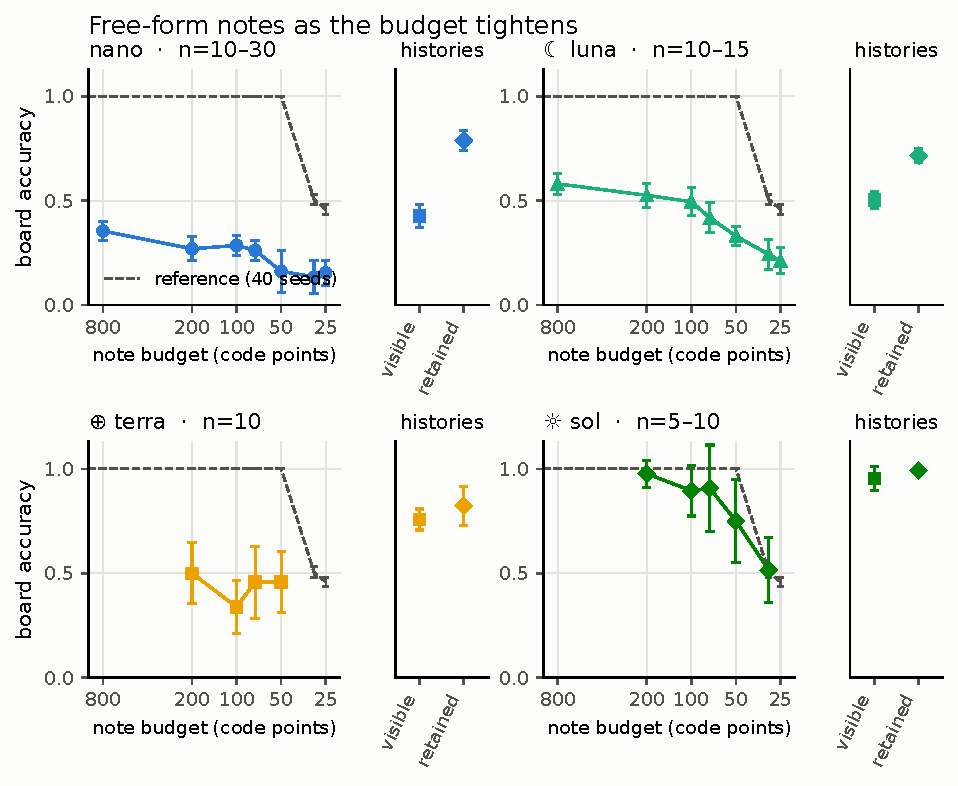
\includegraphics[width=\linewidth]{figures/relay_fig1_knee.pdf}
\caption{Mean board accuracy (fraction of keys correct) with free-form notes and transcript controls for the four original models. Intervals are across-seed 95\% $t$ intervals; cells use all available seeds ($n{=}5$--30; exact counts in \Cref{app:cells}). Numeric budgets follow a descending log axis. Visible and retained histories are separate categorical controls, unconnected to the note-budget curves. Dashed lines show the versioned 40-seed reference mean. These descriptive means do not identify a retention mechanism; the original-model controls span collection dates.}
\label{fig:knee}
\end{figure}

The supplied schema improves Nano's notes by $+\relayprimnanoschematwohundreddelta$ at $B{=}200$ and $+\relayprimnanoschemafiftydelta$ at $B{=}50$. Both survive Holm correction over the declared \relayprimfamily-test family (adjusted $p\relayprimnanoschematwohundredholm$ and $p\relayprimnanoschemafiftyholm$). The $B{=}100$ estimate, $+\relayprimnanoschemahundreddelta$, does not survive correction (adjusted $p\relayprimnanoschemahundredholm$). The harness form also improves scores at $B{=}200$ (adjusted $p\relayprimnanoformtwohundredholm$). These are effects of the supplied interface packages; their role in the model's reasoning is unobserved.

On the separately declared 30-seed comparison at $B{=}100$, schema notes outperform Nano's visible transcript by $+\relayfamtwodelta$ (95\% $t$ CI $[\relayfamtwolo,\relayfamtwohi]$; F2, $p\relayfamtwoholm$). The schema also improves on free-form notes and the visible transcript on the 39-key board (F3). Gemini 3.5 Flash's schema-minus-free-form gain and free-form-minus-visible loss are both unconfirmed after correction (F4; \Cref{tab:families}).

Nano's later retained-reasoning control scores $\relayfamfivestdabs$ above its schema notes (F5; Holm $p\relayfamfivestdholm$) and $\relayfamsevenabs$ above its free-form notes (F7; $p\relayfamsevenp$). These comparisons span collection dates and include any change in the served model. No negative scaffold contrast for the other original models survives family-wise correction (\Cref{tab:contrasts,app:crossover}).

\FloatBarrier

\subsection{Note formats become more similar within long chains}\label{sec:convention}
Luna's notes change notation while remaining compact: \texttt{LMb=A} $\to$ \texttt{Ppt=O} $\to$ \texttt{Lringhome}. We measure this \textbf{notation drift} by comparing consecutive notes after normalizing letters and digits. Similarity then reflects format, length and belief-state shape rather than symbol identity. \Cref{app:format} gives the estimator checks and a complete transmitted sequence.

In Luna's 60-turn-cap runs, mean similarity at successor-note turns 13 onward exceeds similarity at turns 2--7 by $+\relaydriftcleantrendhundred$ at $B{=}100$ (95\% $t$ CI $[\relaydriftcleantrendhundredlo,\relaydriftcleantrendhundredhi]$) and $+\relaydriftcleantrendtwohundred$ at $B{=}200$ ($[\relaydriftcleantrendtwohundredlo,\relaydriftcleantrendtwohundredhi]$). All ten episodes at each budget have a positive difference. This analysis excludes terminal notes, disables the matcher's frequent-character heuristic and averages within episodes before calculating uncertainty.

The within-chain increase survives those checks, but early and late turns also differ in acquired state and rotation exposure. The between-chain metric fails its fixed-codec negative control: reference chains using one notation still become less similar to one another. The evidence therefore supports a surface-format trend, without establishing chain-specific conventions.
\subsection{Retained reasoning improves both Luna controls}\label{sec:retention}
The original four models' retained and visible controls were collected two months apart. Nano's historical retained-minus-visible difference is $+\relayfamsixnanodelta$ (F6; Holm $p\relayfamsixnanoholm$). Luna's estimate is positive but does not survive correction; Terra's and Sol's differences are also unconfirmed (\Cref{tab:families}). These comparisons motivated fresh-seed tests with both controls collected on the same day.

\begin{figure}[htbp]
\centering
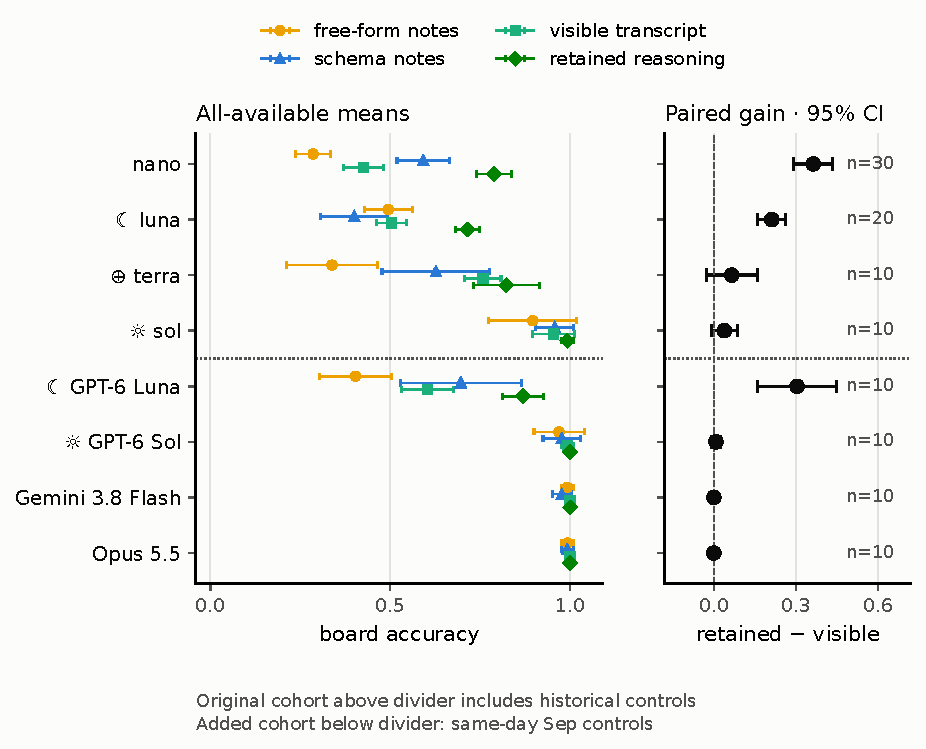
\includegraphics[width=\linewidth]{figures/relay_fig4_models.pdf}
\caption{Board accuracy (fraction of keys correct) across four memory conditions: free-form and schema notes at $B{=}100$, visible transcript and retained reasoning. Left: all-available cell means with across-seed 95\% $t$ intervals, not paired treatment effects. Sample sizes differ; \Cref{app:cells} gives per-cell counts. Right: paired retained-minus-visible differences, with sample sizes shown. Luna pools seeds 0--19 descriptively; its ten-seed F6 test and fresh-seed F8 test are reported separately in \Cref{tab:families}. Nano uses seeds 0--29; all other rows use seeds 0--9. The original four models appear above the dashed line and the four added models below it. Original-model retained controls were collected later. Vertical offsets keep coincident markers visible.}
\label{fig:models}
\end{figure}

Those tests confirm higher retained-reasoning scores for GPT-5.6 Luna and GPT-6 Luna. On ten fresh seeds each, the gains are $+\relayfameightdelta$ (95\% $t$ CI $[\relayfameightlo,\relayfameighthi]$; F8, $p\relayfameightp$) and $+\relayfamthirteendelta$ ($[\relayfamthirteenlo,\relayfamthirteenhi]$; F13, $p\relayfamthirteenp$). The retained control wins on \relayfameightpos{} of \relayfameightn{} seeds for GPT-5.6 Luna and \relayfamthirteenpos{} of \relayfamthirteenn{} for GPT-6 Luna.

\label{sec:added}
\Cref{fig:models} compares the four original models with four added models under the same core interfaces. GPT-6 Luna scores $\relayfamninelunasixabs$ lower with free-form notes than with retained reasoning on the initial ten seeds (F9; 95\% $t$ CI for free-form minus retained $[\relayfamninelunasixlo,\relayfamninelunasixhi]$; Holm $p\relayfamninelunasixholm$). Its schema contrasts are unconfirmed. GPT-6 Sol, Gemini 3.8 Flash and Opus 5.5 score at least $\relayfrontiermin$ in every core condition, leaving little room for improvement. Their unconfirmed contrasts do not establish equivalence, and the cross-model pattern does not establish an interaction between capability and retention.

\FloatBarrier

\subsection{Tighter budgets leave the frontier ranking unresolved}\label{sec:frontier}
At $B{=}50$ on the initial ten seeds, GPT-6 Sol scores $\relayaddfreefiftysolsix$, Opus 5.5 $\relayaddfreefiftyopus$ and Gemini 3.8 Flash $\relayaddfreefiftyflash$ (\Cref{fig:frontier}). At $B{=}30$, each loses about half its retained-control score. Their means lie near the matched reference; GPT-6 Sol's $\relayaddfreethirtysolsix$ is slightly above the reference's $\relayfloorbthirtyshared$. This descriptive proximity does not establish equality.

\begin{figure}[htbp]
\centering
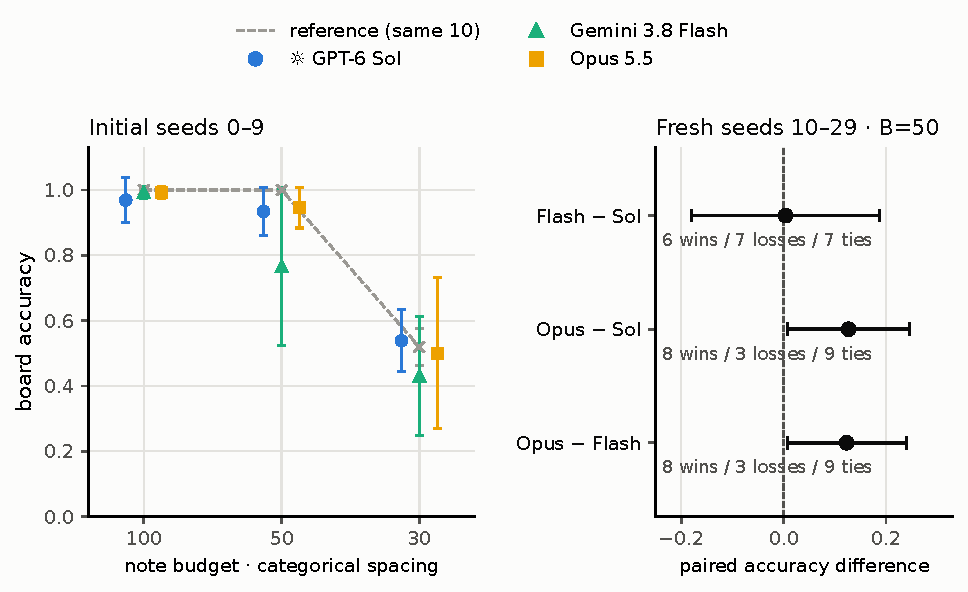
\includegraphics[width=\linewidth]{figures/relay_fig5_frontier.pdf}
\caption{Frontier-model board accuracy (fraction of keys correct) at tighter note budgets. Left: free-form means and across-seed 95\% $t$ intervals for three models and the reference on the same initial ten seeds. Budgets are categorically spaced. At $B{=}30$, GPT-6 Sol scores $\relayaddfreethirtysolsix$, slightly above the matched reference's $\relayfloorbthirtyshared$; equality is not established. Right: paired model differences on fresh seeds 10--29 at $B{=}50$, with 95\% $t$ intervals and sign-test win/loss/tie counts. No pairwise contrast survives the declared family correction (F15/F16).}
\label{fig:frontier}
\end{figure}

Neither the initial pairwise tests nor twenty fresh seeds at $B{=}50$ establish a ranking after correction. The 60-turn-cap condition also leaves the models near the ceiling, with guesses on turns $\relaylongfrontierguessmin$--$\relaylongfrontierguessmax$. It tests a larger available horizon with voluntary stopping. \Cref{app:frontier} gives the complete means, uncertainty, tie counts and family definitions. The pixel-channel results are reported separately in \Cref{app:pixel}.

\FloatBarrier

\subsection{Implications for memory tools}\label{sec:discussion}

The scaffold results support testing each model's memory interface before deployment. A three-condition screen at $B{=}100$---free-form notes, imposed schema and harness form, on ten shared seeds---costs \$\relayfitcostnano{}--\$\relayfitcostsol{} per GPT-5.x model at list prices (\Cref{sec:setup}). Its result is specific to the model, effort, provider and schema. We tested one imposed schema; a second would help distinguish a general benefit of structure from a benefit of this notation.

Multi-turn evaluations should state whether they retain reasoning. The two Luna replications show that this choice can affect scores when both controls retain the full visible transcript. The frontier models remain near the ceiling, where unconfirmed differences reveal little. OpenAI also reports gains from a joint retention-and-compaction change on ARC-AGI-3 \citep{openai2026archarness}; that intervention differs from the replay-only configuration tested here.

\section{Limitations, Ethics, and Reproducibility}\label{sec:limits}

\paragraph{Scale and power.} Most reported cells have $n{=}10$ (\Cref{app:cells}). With ten non-tied seeds, the minimum two-sided exact sign-test value is $2/2^{10}\simeq .00195$, before correction; at least nine wins are needed for raw $\alpha{=}.05$. Ties further limit resolution. Power depends on the alternative and family size, so unconfirmed contrasts establish neither absence nor equivalence. \Cref{sec:setup} specifies the separate test families and their corrections.

\paragraph{Metrics.} Note-format similarity is sensitive to belief-state shape and note length. Early and late turns also differ in state and rotation exposure, so cross-budget trends are descriptive. A fixed-codec negative control prevents interpreting between-chain differences as convention formation (\Cref{sec:convention,app:format}). The syntax classifier counts \texttt{=} or \texttt{:} and undercounts positional strings.

\paragraph{Reasoning state.} Duplicate-lock notices can expose earlier lock status outside the note budget without revealing correctness. We have not measured their effect or repeated collection without them. The retained control tests one provider-native replay configuration (\Cref{sec:setup}); other replay or compaction settings could score differently. Opaque provider representations and token-growth checks establish transport, not semantic use of every earlier thought.

\paragraph{Reference.} The reference is sound, not optimal. The 65- and 97-character peaks are maxima along one policy's 40 evaluated trajectories, not bounds over all states or policies. Character budgets favor boards with single-character symbols. Transfer beyond 26 keys was tested on one board (F3, $n{=}10$).

\paragraph{External validity.} Transfer from a closed 26-fact game to open-world agent memory remains untested. Whether per-model screens predict performance on tasks using notes files or compaction is an open question.

\paragraph{Code and data.} Relay's code, recorded episodes and analysis are available at \url{https://github.com/adamallcock/blindboard-relay}. The base environment, reference solver and harness are available with \blindboard{} \citep{blindboarddata2026}.
% Add the confirmed Relay Zenodo archive citation after archival publication.

\paragraph{Ethics and source safety.} The study involved no human subjects or scraped corpora. All game content is procedurally generated. Task inputs contained no personal data or human-subject records.

\paragraph{AI tool assistance.} AI coding and writing tools assisted with the environment, harness and manuscript. The instrument audit (\Cref{sec:audit}) and all data-collection decisions were made under human direction. The author reviewed all content and takes responsibility for it.

\paragraph{Reproducibility.} The environment trajectory and score can be replayed from the stored actions, configuration, seed and code. Model responses are records, not reproducible generations. Reported results regenerate from \texttt{scripts/relay\_analysis.py}, except the pilot audit figures and hand-built statistics in \Cref{sec:b30,app:pixel}. Census, cost and floor values use generated macros. The paper uses benchkit 0.3.10; the deterministic reference reproduces its calibration exactly. Collection and screen costs are list-price equivalents (\Cref{sec:setup,sec:discussion}).

\section{Conclusion}\label{sec:conclusion}

\relay{} measures whether a model can carry useful memory through budgeted notes between fresh contexts. The budget-matched reference establishes attainable scores. A schema improves Nano's notes; its later retained-reasoning control scores higher still, with collection date as a confound. Same-day tests on fresh seeds confirm retention gains for both Luna models. Tighter budgets do not establish a frontier ranking, and note-format trends do not establish chain-specific conventions. Another schema, more informative frontier instances and an open-world memory task would test how far these findings extend.


\clearpage
\appendix
\crefalias{subsection}{appendix}
\section{Appendix}

\subsection{Detailed score comparisons}\label{app:comparisons}
\Cref{tab:ladder} gives the cell means underlying the main comparisons. \Cref{tab:contrasts} reports the selected primary scaffold tests, \Cref{tab:families} the original-model and fresh-seed confirmatory tests, and \Cref{tab:added} the four added models' initial tests. Means may use more episodes than a declared contrast; each table identifies its own seed population.

\begin{table}[htbp]
\centering
\small
\caption{Mean board accuracy (fraction of keys correct) for core note interfaces at $B{=}100$ and transcript controls. Means use all available episodes; bold marks the largest observed note mean, not a confirmed winner. $n{=}10$ except Luna free-form ($n{=}15$), Luna's and GPT-6 Luna's two transcript controls ($n{=}20$), and Nano free-form, schema and both transcript controls ($n{=}30$). Retained controls also replay earlier reasoning (\Cref{sec:setup}); the original models' retained controls were collected later. The Luna-only constitution case is reported separately; the added models have no form cell. \Cref{app:cells} gives per-cell counts.}
\label{tab:ladder}
% Generated by scripts/relay_analysis.py. Do not hand-edit.
\begin{tabular}{@{}lrrrrr@{}}
\toprule
 & \multicolumn{3}{c}{note at $B{=}100$} & \multicolumn{2}{c}{transcript control} \\
\cmidrule(lr){2-4}\cmidrule(l){5-6}
model & free-form & schema & form & visible & retained \\
\midrule
nano & .286 & \textbf{.592} & .523 & .426 & .788 \\
\lunaicon\ luna & .495 & .400 & \textbf{.500} & .504 & .715 \\
\terraicon\ terra & .338 & \textbf{.627} & .319 & .758 & .823 \\
\solicon\ sol & .896 & \textbf{.958} & .642 & .954 & .992 \\
\midrule
\multicolumn{6}{@{}l}{\textit{Added models, seeds 0--9 (GPT-6 Luna's transcripts 0--19)}} \\
\lunaicon\ GPT-6 Luna & .404 & \textbf{.696} & -- & .604 & .869 \\
\solicon\ GPT-6 Sol & .969 & \textbf{.977} & -- & .992 & 1.000 \\
Gemini 3.8 Flash & \textbf{.992} & .977 & -- & 1.000 & 1.000 \\
Opus 5.5 & \textbf{.992} & \textbf{.992} & -- & 1.000 & 1.000 \\
\bottomrule
\end{tabular}

\end{table}

\begin{table}[htbp]
\centering
\small
\caption{Selected paired differences in board accuracy (fraction of keys correct; condition $-$ free-form) from the declared primary family of \relayprimfamily{} scaffolding tests, using seeds 0--9 ($n{=}10$). Holm correction uses the full family. Sign tests are exact and two-sided. Signed-rank $p$ values use midranks of integer correct-key differences as a sensitivity check. Rows include every Nano schema contrast, every contrast that survives correction, and the other $B{=}100$ contrasts. The remaining \relayprimhidden{} rows are in \texttt{analysis.json}.}
\label{tab:contrasts}
% Generated by scripts/relay_analysis.py. Do not hand-edit.
% Family: all 24 computed contrasts; Holm and BH adjusted over that family.
\begin{tabular}{@{}llrrrrrrr@{}}
\toprule
model & condition & $B$ & $n$ & $\Delta$ & 95\% $t$ CI & sign $p$ & signed-rank $p$ & Holm $p$ \\
\midrule
nano & schema & 200 & 10 & $+.419$ & $[+.304, +.535]$ & \phantom{<}.002 & \phantom{<}.002 & \phantom{<}.047 \\
 & schema & 100 & 10 & $+.381$ & $[+.256, +.505]$ & \phantom{<}.004 & \phantom{<}.004 & \phantom{<}.082 \\
 & schema & 75 & 10 & $+.385$ & $[+.199, +.570]$ & \phantom{<}.109 & \phantom{<}.010 & 1.000 \\
 & schema & 50 & 10 & $+.512$ & $[+.384, +.639]$ & \phantom{<}.002 & \phantom{<}.002 & \phantom{<}.047 \\
 & form & 200 & 10 & $+.377$ & $[+.254, +.500]$ & \phantom{<}.002 & \phantom{<}.002 & \phantom{<}.047 \\
 & form & 100 & 10 & $+.208$ & $[+.119, +.297]$ & \phantom{<}.021 & \phantom{<}.004 & \phantom{<}.430 \\
\addlinespace
\lunaicon\ luna & schema & 100 & 10 & $-.081$ & $[-.223, +.062]$ & \phantom{<}.727 & \phantom{<}.203 & 1.000 \\
 & form & 100 & 10 & $+.019$ & $[-.107, +.145]$ & 1.000 & \phantom{<}.613 & 1.000 \\
 & constitution & 100 & 10 & $-.142$ & $[-.250, -.035]$ & \phantom{<}.109 & \phantom{<}.027 & 1.000 \\
\addlinespace
\terraicon\ terra & schema & 100 & 10 & $+.288$ & $[+.153, +.424]$ & \phantom{<}.021 & \phantom{<}.004 & \phantom{<}.430 \\
 & form & 100 & 10 & $-.019$ & $[-.180, +.142]$ & \phantom{<}.508 & \phantom{<}.816 & 1.000 \\
\addlinespace
\solicon\ sol & schema & 100 & 10 & $+.062$ & $[-.067, +.190]$ & \phantom{<}.219 & \phantom{<}.344 & 1.000 \\
 & form & 100 & 10 & $-.254$ & $[-.370, -.138]$ & \phantom{<}.021 & \phantom{<}.006 & \phantom{<}.430 \\
\bottomrule
\end{tabular}

\end{table}

\begin{table}[htbp]
\centering
\small
\setlength{\tabcolsep}{4pt}
\caption{Prospectively declared confirmatory families, each declared before its own data collection and Holm-corrected within itself. $\Delta$ is the paired difference in board accuracy (fraction of keys correct), first condition minus second; $n$ counts paired seeds. Note conditions use $B{=}100$. Visible and retained denote the transcript controls (\Cref{sec:setup}); 39-key denotes the transfer board. F9--F12 and F14--F17 for the added models appear in \Cref{tab:added,tab:frontier}.}
\label{tab:families}
% Generated by scripts/relay_analysis.py. Do not hand-edit.
\begin{tabular}{@{}lllrrrrr@{}}
\toprule
family & model & contrast & $n$ & $\Delta$ & 95\% $t$ CI & sign $p$ & Holm $p$ \\
\midrule
F2 & nano & schema $-$ visible & 30 & $+.167$ & $[+.072, +.262]$ & \phantom{<}.013 & \phantom{<}.013 \\
\addlinespace
F3 & nano & schema $-$ free-form (39-key) & 10 & $+.310$ & $[+.207, +.413]$ & \phantom{<}.021 & \phantom{<}.043 \\
 & nano & schema $-$ visible (39-key) & 10 & $+.192$ & $[+.072, +.312]$ & \phantom{<}.039 & \phantom{<}.043 \\
\addlinespace
F4 & Gemini 3.5 Flash & free-form $-$ visible & 10 & $-.212$ & $[-.454, +.031]$ & \phantom{<}.289 & \phantom{<}.289 \\
 & Gemini 3.5 Flash & schema $-$ free-form & 10 & $+.254$ & $[+.022, +.486]$ & \phantom{<}.031 & \phantom{<}.062 \\
\addlinespace
F5 & nano & schema $-$ retained & 30 & $-.196$ & $[-.295, -.097]$ & <.001 & \phantom{<}.001 \\
 & nano & schema $-$ retained (39-key) & 10 & $-.087$ & $[-.199, +.024]$ & \phantom{<}.109 & \phantom{<}.109 \\
\addlinespace
F6 & nano & retained $-$ visible & 30 & $+.363$ & $[+.292, +.434]$ & <.001 & <.001 \\
 & \lunaicon\ luna & retained $-$ visible & 10 & $+.204$ & $[+.123, +.285]$ & \phantom{<}.021 & \phantom{<}.064 \\
 & \terraicon\ terra & retained $-$ visible & 10 & $+.065$ & $[-.027, +.158]$ & \phantom{<}.180 & \phantom{<}.359 \\
 & \solicon\ sol & retained $-$ visible & 10 & $+.038$ & $[-.010, +.087]$ & \phantom{<}.250 & \phantom{<}.359 \\
\addlinespace
F7 & nano & free-form $-$ retained & 30 & $-.503$ & $[-.577, -.428]$ & <.001 & <.001 \\
\addlinespace
F8 & \lunaicon\ luna & retained $-$ visible (fresh seeds 10--19) & 10 & $+.219$ & $[+.138, +.300]$ & \phantom{<}.002 & \phantom{<}.002 \\
\addlinespace
F13 & \lunaicon\ GPT-6 Luna & retained $-$ visible (fresh seeds 10--19) & 10 & $+.227$ & $[+.111, +.343]$ & \phantom{<}.021 & \phantom{<}.021 \\
\bottomrule
\end{tabular}

\end{table}

\begin{table}[htbp]
\centering
\small
\caption{Paired differences in board accuracy (fraction of keys correct) for the four added models, with $n{=}10$ shared seeds per row. Note conditions use $B{=}100$. Each declared family is Holm-corrected over its four model rows. F9: free-form notes $-$ retained reasoning (F7's comparison). F10: schema $-$ free-form notes. F11: schema $-$ retained reasoning (F5's comparison). F12: retained reasoning $-$ visible transcript (F6's comparison).}
\label{tab:added}
% Generated by scripts/relay_analysis.py. Do not hand-edit.
\begin{tabular}{@{}lrrrrrrrr@{}}
\toprule
 & \multicolumn{2}{c}{F9} & \multicolumn{2}{c}{F10} & \multicolumn{2}{c}{F11} & \multicolumn{2}{c}{F12} \\
\cmidrule(lr){2-3}\cmidrule(lr){4-5}\cmidrule(lr){6-7}\cmidrule(lr){8-9}
model & $\Delta$ & Holm $p$ & $\Delta$ & Holm $p$ & $\Delta$ & Holm $p$ & $\Delta$ & Holm $p$ \\
\midrule
\lunaicon\ GPT-6 Luna & $-.473$ & \phantom{<}.008 & $+.292$ & \phantom{<}.438 & $-.181$ & \phantom{<}.719 & $+.304$ & \phantom{<}.086 \\
\solicon\ GPT-6 Sol & $-.031$ & 1.000 & $+.008$ & 1.000 & $-.023$ & 1.000 & $+.008$ & 1.000 \\
Gemini 3.8 Flash & $-.008$ & 1.000 & $-.015$ & 1.000 & $-.023$ & \phantom{<}.750 & $+.000$ & 1.000 \\
Opus 5.5 & $-.008$ & 1.000 & $+.000$ & 1.000 & $-.008$ & 1.000 & $+.000$ & 1.000 \\
\bottomrule
\end{tabular}

\end{table}

The primary family uses seeds 0--9 throughout. Nano's later seeds 10--29 are included only in the separately declared comparisons and all-available descriptive means. Thus its $B{=}100$ schema row has $n{=}10$ in \Cref{tab:contrasts} and $n{=}30$ in \Cref{tab:ladder}.

Terra's free-form scores are below its visible-transcript mean at every measured budget ($\relayterranotemin$--$\relayterranotemax$ versus $\relayterrafullmean$). Its average loss across the four budgets shared with Nano is larger by $\relayterraexcess$, but the paired-seed interval crosses zero (95\% CI $[\relayterraexcesslo,\relayterraexcesshi]$; exact sign $p\relayterraexcessp$; $n{=}\relayterraexcessn$). This does not establish a cross-model difference.

Against the retained-reasoning control, only Sol among the original four preserves 80\% of its score across binding note budgets, down to $B{=}\relayfullmemsolfloor$. Luna reaches that threshold only at $B{=}800$ ($\relaylunaeighthundred$ against a threshold of $\relayfullmemlineluna$). Nano and Terra fall short at every tested budget.

\FloatBarrier

\subsection{Per-cell episode counts (generated)}\label{app:cells}
% Not a float: the table is this appendix's only content, so it stays under
% the heading (and moves with it) instead of drifting away from it. One
% minipage cannot break, so the caption never parts from the table body.
\noindent\begin{minipage}{\linewidth}\centering\small
\captionsetup{hypcap=false}% the link target is the caption itself (not a float)
\captionof{table}{Episode count $n$ for every reported text-channel cell, separated by prompt version and generated from the stored corpus by \texttt{scripts/\allowbreak relay\_analysis.py}. Transcript controls appear on the free-form rows; \texttt{std} denotes the 26-key relay base with a 20-turn cap. Uncollected cells have no reported count. Standard and long conditions allow at most 20 and 60 turns, respectively; early guesses are permitted.}
\label{tab:cells}
% Generated by scripts/relay_analysis.py. Do not hand-edit.
\begin{tabular}{@{}lllrrrrrrrrr@{}}
\toprule
 & & & \multicolumn{2}{c}{transcript control} & \multicolumn{7}{c}{note budget $B$ (characters)} \\
\cmidrule(l{2pt}r{2pt}){4-5}\cmidrule(l{2pt}r{2pt}){6-12}
model & condition & base & visible & retained & 800 & 200 & 100 & 75 & 50 & 30 & 25 \\
\midrule
\multicolumn{12}{@{}l}{\textit{Main grid: relay-v2 prompt}} \\
nano & free-form & std & 30 & 30 & 30 & 10 & 30 & 10 & 10 & 10 & 10 \\
 & free-form & 39-key & 10 & 10 &  &  & 10 &  &  &  &  \\
 & schema & std &  &  &  & 10 & 30 & 10 & 10 &  &  \\
 & schema & 39-key &  &  &  &  & 10 &  &  &  &  \\
 & form & std &  &  &  & 10 & 10 & 10 & 10 &  &  \\
\addlinespace
\lunaicon\ luna & free-form & std & 20 & 20 & 10 & 15 & 15 & 15 & 15 & 10 & 10 \\
 & free-form & 60-turn &  &  &  & 10 & 10 &  &  &  &  \\
 & schema & std &  &  &  & 10 & 10 & 10 & 10 &  &  \\
 & constitution & std &  &  &  & 10 & 10 & 10 & 10 &  &  \\
 & form & std &  &  &  & 10 & 10 & 10 & 10 &  &  \\
\addlinespace
\terraicon\ terra & free-form & std & 10 & 10 &  & 10 & 10 & 10 & 10 &  &  \\
 & schema & std &  &  &  &  & 10 &  &  &  &  \\
 & form & std &  &  &  &  & 10 &  &  &  &  \\
\addlinespace
\solicon\ sol & free-form & std & 10 & 10 &  & 5 & 10 & 5 & 10 & 10 &  \\
 & schema & std &  &  &  &  & 10 &  &  &  &  \\
 & form & std &  &  &  &  & 10 &  &  &  &  \\
\addlinespace
Gemini 3.8 Flash & free-form & std & 10 & 10 &  &  & 10 &  & 30 & 10 &  \\
 & free-form & 60-turn &  &  &  &  & 10 &  &  &  &  \\
 & schema & std &  &  &  &  & 10 &  &  &  &  \\
\addlinespace
Gemini 3.5 Flash & free-form & std & 10 &  &  &  & 10 &  &  &  &  \\
 & schema & std &  &  &  &  & 10 &  &  &  &  \\
\addlinespace
\lunaicon\ GPT-6 Luna & free-form & std & 20 & 20 &  &  & 10 &  &  &  &  \\
 & schema & std &  &  &  &  & 10 &  &  &  &  \\
\addlinespace
Opus 5.5 & free-form & std & 10 & 10 &  &  & 10 &  & 30 & 10 &  \\
 & free-form & 60-turn &  &  &  &  & 10 &  &  &  &  \\
 & schema & std &  &  &  &  & 10 &  &  &  &  \\
\addlinespace
\solicon\ GPT-6 Sol & free-form & std & 10 & 10 &  &  & 10 &  & 30 & 10 &  \\
 & free-form & 60-turn &  &  &  &  & 10 &  &  &  &  \\
 & schema & std &  &  &  &  & 10 &  &  &  &  \\
\midrule
\multicolumn{12}{@{}l}{\textit{Audit cells: \texttt{nocoach} prompt variant (relay-v3-nocoach), loaded separately}} \\
nano & free-form & std &  &  &  &  & 10 &  &  &  &  \\
\lunaicon\ luna & free-form & std &  &  &  &  & 10 &  &  &  &  \\
\terraicon\ terra & free-form & std &  &  &  &  & 10 &  &  &  &  \\
\solicon\ sol & free-form & std &  &  &  &  & 10 &  &  &  &  \\
\bottomrule
\end{tabular}

\end{minipage}

\subsection{Note-format diagnostics and examples}\label{app:format}\label{app:drift}
Luna's free-form operational 80\%-retention crossing (\Cref{sec:reference}) is $B{=}\relaycrossingluna$. Its mean there is $\relaycrosscellluna$, compared with $\relaycrosslineluna$, the 80\% threshold for its visible transcript. The sound reference crosses at $B{=}\relayrefcrossing$. The ratio of these observed budgets is $\sim$\relaytaxluna$\times$, the same as Sol's under this convention. At $B{=}50$, Luna scores $.331$ while the reference scores $1.000$.

Luna's notes remain compact while their notation changes: \texttt{LMb=A} $\to$ \texttt{Ppt=O} $\to$ \texttt{Lringhome}. We call this \textbf{notation drift}. The sequence below shows six complete transmitted notes. To measure surface similarity without retaining symbol identities, we map letters$\to$\texttt{A}/\texttt{a} and digits$\to$\texttt{0}, retain punctuation, and compare consecutive note skeletons by sequence similarity. There are \relaydriftpairsstd{} pairs in the 20-turn cells and \relaydriftpairsall{} including the 60-turn-cap cells. Renaming symbols leaves the metric unchanged, but changes in the shape of the underlying belief state can alter it.

\begin{table}[htbp]
\centering
\small
\caption{Descriptive note-format metrics for free-form notes at $B{=}100$. Similarity is the historical mean over adjacent nonempty, letter/digit-normalized note pairs, using \texttt{SequenceMatcher(autojunk=True)}. The syntax share is the fraction of notes containing \texttt{=} or \texttt{:}; it does not verify factual content. $n$ counts episodes; pair counts and nonempty-note counts give the separate denominators. The text reports sensitivity to the estimator and terminal-note inclusion.}
\label{tab:drift}
% Generated by scripts/relay_analysis.py. Do not hand-edit.
\begin{tabular}{@{}lrrrrrr@{}}
\toprule
model & $n$ & pairs & similarity & notes & \texttt{=} or \texttt{:} & plan-only \\
\midrule
nano & 30 & 566 & .564 & 596 & .95 & .02 \\
\lunaicon\ luna & 15 & 281 & .691 & 296 & .97 & .02 \\
\terraicon\ terra & 10 & 185 & .695 & 195 & .85 & .02 \\
\solicon\ sol & 10 & 170 & .677 & 180 & .93 & .02 \\
\bottomrule
\end{tabular}

\end{table}

The historical estimator used Python's \texttt{SequenceMatcher} with \texttt{autojunk=True}. This setting suppresses frequent characters in strings of at least 200 elements and materially affects cross-budget comparisons. On the same recorded pairs, disabling it raises Luna's $B{=}800$ mean from $\relaydriftampleluna$ to $\relaydriftcleanampleluna$ and Nano's from $\relaydriftamplenano$ to $\relaydriftcleanamplenano$. The $B{=}25$ values remain $\relaydriftcleanscarceluna$ and $\relaydriftcleanscarcenano$. The ordering remains, but these length-sensitive measurements do not establish scarcity-driven standardization.

The between-chain metric fails a fixed-codec negative control. Reference chains that share one notation still show a late decline in similarity. Their historical decline is $\relaynegcontrol$, compared with Luna's $\relaybetweenlunahundred$ and $\relaybetweenlunatwohundred$. The generated control is retained in \texttt{results/relay/calibration/negative-control.json}; \texttt{analysis.json} retains the original estimator and versioned sensitivity analysis. The within-chain trend survives the estimator checks, but the evidence does not establish chain-specific convention formation. \Cref{sec:convention} reports the corrected within-chain changes; \Cref{app:lockin} reports the pinned-notation case study.

Nano's notes usually contain fact-like syntax: \relaystatepctnano\% of its $B{=}100$ notes contain the markers counted in \Cref{tab:drift}. Notes classified as plan-only are rare for every model ($\leq$\relayplanpctmax\%). Nano has the least stable note format in the original family. Consecutive-note similarity at $B{=}100$ is $\relaydriftsimnano$, compared with Luna's $\relaydriftsimluna$. Mean normalized note lengths are comparable (\relaydriftlennano{} versus \relaydriftlenluna{} skeleton characters). This reduces one length difference without separating notation from belief-state shape. Sampled notes still contain plan-shaped failures (``T19 press LrT... deduce from remaining''), but the quantitative pattern is unstable formatting rather than an absence of fact-like syntax. Format instability is a possible explanation for the lower scores, not an established cause.

Luna guessed on turns $\relaylonglunahundredguessmin$--$\relaylonglunahundredguessmax$ at $B{=}100$ and $\relaylonglunatwohundredguessmin$--$\relaylonglunatwohundredguessmax$ at $B{=}200$ in the 60-turn-cap condition.

\noindent\begin{minipage}{\linewidth}
\paragraph{Six consecutive transmitted notes.}
These are the complete transmitted notes from turns 4--9 of one main-v2 episode: GPT-5.6 Luna, free-form notes, $B{=}100$, seed 0. Truncated endings are preserved exactly. Source: \path{results/relay/llm/gpt-5.6-luna-medium-freeform-b100-20260714-180239/seed0000.json}. The notes illustrate one sequence; they are neither a semantic classification nor a representative random sample.
% Generated by scripts/relay_analysis.py. Do not hand-edit.
\begin{quote}\small\ttfamily\raggedright
\textnormal{Turn 4:} Known now: LrH=L; LpT/LpH=\{Y,Z\}, LpB=M before rotation. Query LpT,LpH,LrH,LmT; rotations may alter l\par\medskip
\textnormal{Turn 5:} Known current: LrH=L, LmT=O; LpT/LpH=\{Y,Z\}. Query LpT+LrH+LmT+L-index-top to resolve pinky and index\par\medskip
\textnormal{Turn 6:} Known: LpT=Y, LpH=Z, LrH=L, LmT=O, LiT=A. Query LiH with Y,L,O.\par\medskip
\textnormal{Turn 7:} Known LpT=Y,LrH=L,LiH=X,LmT=O. Queried LrT with Y,L,X; identify its 4th symbol. LpH/RrT rotation unr\par\medskip
\textnormal{Turn 8:} Known current: LpT=Y,LrH=L,LiH=X,LrT=M. Query LpH via Y,L,X,LpH; LmT/RiHi rotated.\par\medskip
\textnormal{Turn 9:} Known current: LpT=Y,LrH=L,LiH=X,LpH=F,LrT=M. Query LmT with Y,L,X.\par\medskip
\end{quote}

\end{minipage}

\FloatBarrier

\subsection{Channel rules as delivered (verbatim, unelided)}\label{app:prompts}
The following is the complete v2 relay-mode block appended to the base-game rules. The value of \texttt{\{budget\}} is substituted for each cell. The final two sentences form the coaching block evaluated in \Cref{tab:audit}. The \texttt{nocoach} variant removes exactly those two sentences; no text is elided here.
\begin{quote}\small\ttfamily
RELAY MODE \textemdash{} READ CAREFULLY\\
You have NO memory of previous turns. Every turn is played by a fresh instance of you: this message is literally everything you know. There is no transcript and no way to see past observations.\\[3pt]
The ONLY thing that survives between turns is a NOTE that you write. The note you receive below was written by you, one turn ago, for you. The note you write now is the only information your next turn's self will have (besides these rules and that turn's fresh observation).\\[3pt]
Notes do NOT accumulate: your successor receives ONLY the single note you write this turn. The note shown below is destroyed after this turn \textemdash{} whatever from it still matters must be carried in your own note.\\[3pt]
Your successor's observation will automatically include the presses you make this turn, the symbols they produce, and any rotation notice \textemdash{} exactly like the observation you see below.\\[3pt]
Add a "note" field to your action JSON: \{"presses": [...], "note": "..."\}. HARD LIMIT: this turn's note budget is \{budget\} characters \textemdash{} anything beyond that is torn off and lost forever. Do not waste characters on prose, apologies, or restating the rules (your successor has the rules). \emph{Invent the densest notation you can and keep it consistent so your future self can decode it. Record what matters: what you know about the layout, what is still uncertain, and what you were planning.}
\end{quote}

\noindent\begin{minipage}{\linewidth}
\paragraph{Imposed-schema notation.}
The schema condition adds the following block verbatim, with \texttt{\{key\_range\}} substituted for each board.
\begin{quote}\small\ttfamily
NOTE NOTATION (required)\\
Write your note in this exact notation. Keys are numbered in the order of the address list above: \{key\_range\} (so key 0 = the first address, key a = the 11th). Two entry types, concatenated with no spaces:\\
\hspace*{1em}!<key><SYM><key><SYM>...\hspace{2em}known keys, e.g. !3Q7A means key 3 = Q, \mbox{key 7 = A}\\
\hspace*{1em}|<keys>:<SYMS>\hspace{5.5em}a set fact, e.g. |58h:BKM means keys 5,8,h hold \{B,K,M\} in some order\\
Example note: !3Q7A|58h:BKM
\end{quote}
\end{minipage}

\subsection{GPT-5.6 Sol and the reference floor (exploratory)}\label{sec:b30}
At $B{=}50$, Sol scores $.750$ ($n{=}10$), 25 percentage points below the sound reference's $1.000$. Under the operational 80\%-retention definition in \Cref{sec:reference}, Sol crosses at $B{=}75$. Sol therefore needs $\sim$1.5$\times$ the reference's threshold budget; their crossings do not match. At $B{=}30$, Sol scored $\relaysolbthirty$ and the reference scored $.519$ on the same ten seeds; the archived 40-seed reference mean is $\relayfloorbthirty$. The paired estimate was $\Delta{=}{-}.004$ (95\% $t$ CI $[-.143,+.136]$; exact sign $p{=}.754$). This post-hoc comparison is too imprecise to establish that Sol meets the reference floor. Equivalence within $\pm.10$ is not demonstrated (two one-sided tests, $p{=}.077$).

Sol's $B{=}50$ notes contain a self-generated \textbf{positional-string encoding}: one character per key in address order, with \texttt{?} for unknowns. A full layout takes 26 characters, compared with 53 in our entry codec. We adopted the encoding into the reference codec and re-certified it. Observing the encoding at $B{=}50$ also prompted the choice of $B{=}30$ (\Cref{sec:channels}), so this original Sol comparison is exploratory. The dual-codec calibration in \Cref{sec:reference} shows that adoption did not raise the $B{=}30$ floor used for comparison, even though the model's encoding prompted the comparison itself. At $B{=}30$, Sol's positional attempts are frequently corrupted: 2/10 episodes contain clean signatures. The layout alone requires 26 of the 30 characters, leaving little room for other content.

\noindent Verbatim examples from Sol:\\
$B{=}50$, turn 19 (episode solved 26/26):\\
\texttt{OJNYFCUBALMHKQTSVIEDZ?R???;ioWX;lpGP}\\[3pt]
$B{=}30$: \texttt{OJNYFCUBaKMHLQTSba?ddX????OQZV}\\
\emph{(case corruption within the 26-of-30-character margin)}

\subsection{The pixel channel: transcription fidelity and game performance (exploratory)}\label{app:pixel}

\begin{table}[htbp]
\centering
\small
\caption{SVG transcription-probe recovery and game performance (rendering and probe protocol in \Cref{sec:channels}). Recall and precision are macro-averaged over 12 probe pairs per model, with invalid writes scored as zero. Game accuracy is the fraction of keys correct; episode counts appear in the final column. Probe and game validity use the separate write counts shown. The results do not separate writing from reading errors or identify the cause of game-performance differences.}
\label{tab:svg}
\begin{tabular}{@{}lrrrrr@{}}
\toprule
 & \multicolumn{3}{c}{transcription probe (12 pairs)} & \multicolumn{2}{c}{game} \\
\cmidrule(lr){2-4}\cmidrule(l){5-6}
model & valid writes & recall & precision & SVG valid & accuracy \\
\midrule
\solicon\ sol & 12/12 & 1.000 & 1.000 & 1.000 (97/97) & .608 ($n{=}5$) \\
nano & 12/12 & .667 & .746 & .995 (199/200) & .304 ($n{=}10$) \\
\lunaicon\ luna & 7/12 & .575 & .583 & 1.000 (199/199) & .335 ($n{=}10$) \\
\bottomrule
\end{tabular}
\end{table}

\begin{figure}[!ht]
\centering
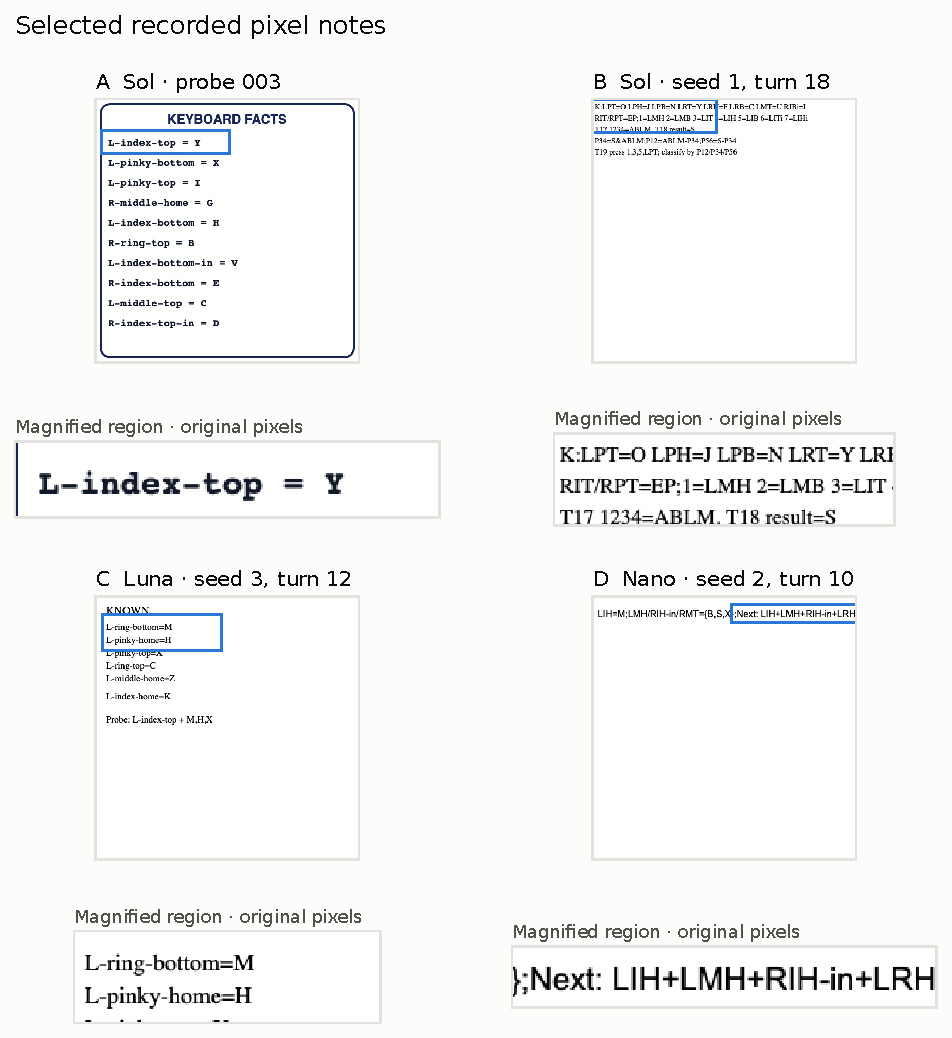
\includegraphics[width=\linewidth]{figures/relay_fig2_svg_notes.pdf}
\caption{Four selected stored pixel notes: a GPT-5.6 Sol transcription probe (A) and game notes from Sol (B), GPT-5.6 Luna (C) and GPT-5.4 Nano (D). Insets magnify the original pixels. Sol's titled, monospaced probe card was recovered without error; Luna's larger text leaves less room for content; Nano's single line clips at the canvas edge. These text-bearing examples do not establish whether spatial encoding strategies occur elsewhere in the corpus.}
\label{fig:svgnotes}
\end{figure}

Sol's perfect write--render--read recovery on the probe coexists with a lower game-score estimate. On the five shared seeds, SVG accuracy is $.608$ and $B{=}100$ text accuracy is $.923$, a paired difference of $-.32$ (\Cref{tab:svg}). The SVG cap of 2{,}500 bytes has no single equivalent text budget, so this is not a capacity-matched comparison. The game cell has $n{=}5$, and the SVG-minus-text contrast is unconfirmed (exact sign $p{=}.375$). Terra and the four added models were not tested in this channel.

The probe contains 10 independent facts, not mid-game set constraints. It differs from the game in both state complexity and query demand. Perfect recovery on this simpler probe does not explain the lower game point estimate or identify its cause. Both image and text interfaces require a replacement artifact on every turn. The selected images show self-authored text layouts; we did not classify spatial strategies across the corpus. These small-sample channel comparisons remain underpowered.

\subsection{Paired scaffold contrasts and pinned notation (exploratory)}\label{app:crossover}

Two different treatments have negative estimates at raw $p{=}.021$ (\Cref{tab:contrasts}): the schema for Luna ($-.22$ at $B{=}200$) and the form for Sol ($-.25$ at $B{=}100$). Neither survives family-wise correction. Sol's schema estimate is positive, as is Terra's (\Cref{tab:contrasts}). These results do not establish that imposed schemas harm stronger models as a class.

Luna's schema estimates are negative at every tested budget. One possible explanation is the need to translate between mnemonic addresses and key indices. A compact notation need not be easy for the model to use, and Luna's better-performing notes retain readable mnemonic addresses. The harness form also replaces Sol's existing strategy. These observations suggest possible mechanisms but do not identify one; at $n{=}10$, none of these contrasts survives correction. A follow-up is inexpensive: the three-condition screen at $B{=}100$ costs \$\relayfitcostnano--\$\relayfitcostsol{} per model at list prices. A confirmatory study would need a declared effect, power calculation and stopping rule.

\begin{figure}[!ht]
\centering
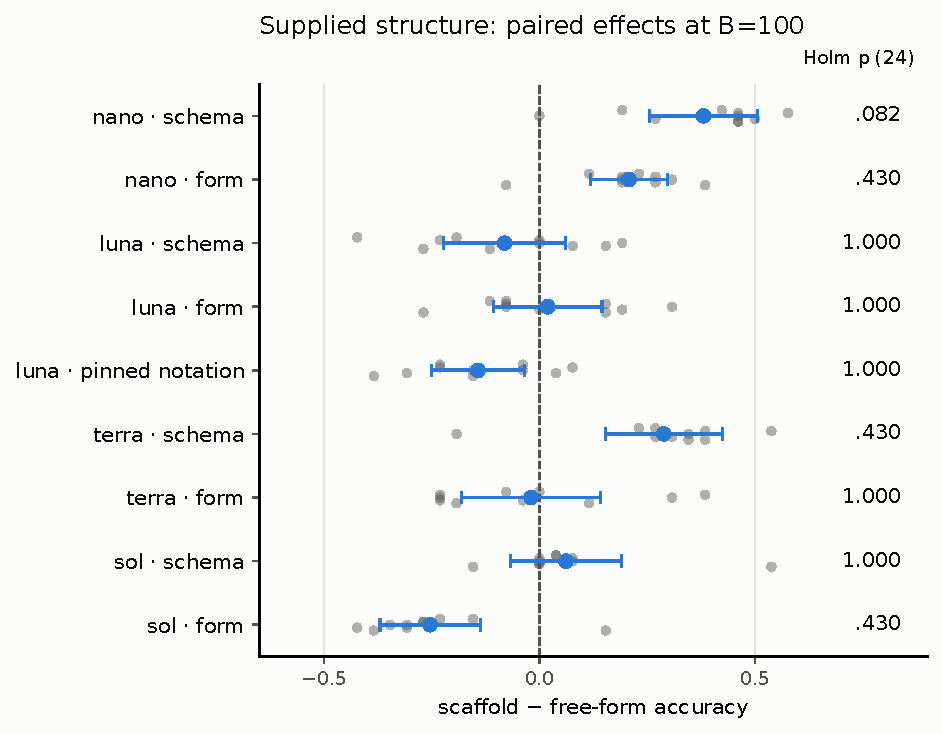
\includegraphics[width=\linewidth]{figures/relay_fig3_crossover.pdf}
\caption{Paired scaffold-minus-free-form differences in board accuracy (fraction of keys correct) at $B{=}100$, using seeds 0--9 ($n{=}10$). Points show mean and individual seed differences; intervals are 95\% $t$ intervals. Holm $p$ values use the full declared 24-test family. The pinned-notation row is for GPT-5.6 Luna only. These compare interface packages, not a cross-model interaction; no negative contrast survives family correction.}
\label{fig:crossover}
\end{figure}

\paragraph{Pinned-notation case study.}\label{app:lockin}
Designing a notation before play did not establish a benefit for the one model tested. Luna's pinned specification, the \emph{constitution} condition, has a lower mean than free-form notes at three of four budgets. Estimates range from $-.16$ to $+.01$; the smallest raw $p{=}.109$, and none survives correction. Luna designs specifications of 258--400 characters for note budgets of 50--200 (\Cref{app:constitution}), but the specification itself is outside the note budget. Its length therefore does not establish that the design is infeasible. A persistent but suboptimal convention is a possible explanation, not an identified mechanism. This is a single-model case study with unconfirmed differences.

\subsection{A constitution, verbatim (GPT-5.6 Luna; designed for \texorpdfstring{$B{=}100$}{B=100})}\label{app:constitution}
\begin{quote}\footnotesize\ttfamily\raggedright\sloppy
Keys are coded 0\textendash{}9,A\textendash{}P in the board-list order. Note format: `m=XXXXXXXXXXXXXXXXXXXXXXXXXX` (current key$\to$letter; `.` unknown); `h=abcd/EFGH` entries record each chord's 4 key codes and sorted result, newest first; append `!xyz` for rotated keys. Delete entries proven redundant. `q=abcd` is next planned chord; `l=` records locks. Use $\leq$100 chars.
\end{quote}
The \texttt{m=} layout field uses 28 characters and fits the 100-character note budget. The specification itself is free. It gives no separate bound for history entries and does not fully specify how to limit the auxiliary history and planning fields. The observed score comparisons do not establish a benefit from pinning the specification.

\FloatBarrier

\subsection{Interpretation and remaining experiments}\label{app:interpretation}
The declared tests do not resolve the frontier-model comparisons. A ranking requires enough informative paired instances to detect the intended differences, not necessarily a condition below the ceiling on every seed. For the frontier models, the 39-key board at $B{=}100$ remains an unrun candidate. The reference's full-state serialization peaked at 97 characters on its evaluated trajectories; that does not predict difficulty for frontier models.

Transmission chains motivate the note-format diagnostics \citep{kirby2001,kirby2008,acerbi2023,telephone2024,brokentelephone2025}. Fixed model weights do not rule out in-context adaptation, and we did not identify attractor dynamics or a cultural-evolution mechanism. A cross-model reader test and a representation that passes the fixed-codec negative control could test stronger claims about conventions.

Reference improvements must remain versioned. A fixed policy's attainable score can be exceeded. Adopting a model's encoding into a later codec does not revise that model's result against the earlier version. Both calibration generations are retained. Extending the protocol to another benchmark with a sound player remains a proposal.

\subsection{Extended related work}\label{app:related}

\paragraph{Agent memory: benchmarks and architectures}
Agent-memory benchmarks evaluate recall in a persistent agent's accumulating context or memory store: long conversations \citep{locomo2024}, multi-platform enterprise timelines \citep{memtrack2025}, dynamic environments \citep{gaia226,evoarena2026}, multi-session applications \citep{memoryarena2026,memgym2026}, and staleness detection \citep{stale2026}. Staleness detection shares \blindboard's premise that retrieving a fact does not establish whether it is still current. Relay resets the context on every turn and measures performance when the model must write the note that preserves its authored memory.

\citet{signals2026} vary memory architecture in a Lewis signaling game, a cooperative coordination task. They compare an overwritten 150-word scratchpad, fixed-capacity codebooks and a rolling 20-round history, and report that stateless agents' performance collapses at high channel capacity. This shows the importance of what is passed between calls, but the task requires neither hidden-state deduction nor budget certification and does not compare a ladder of scaffolds. Latent ``relay'' compression \citep{kvrelay2026} passes continuous key--value (KV) cache state between agents at specified compression ratios. The artifact is sub-symbolic, so there is no explicit notation to invent, inspect or track as it changes, as there is in Relay's human-legible channel.

A rate-distortion account of agent memory \citep{ratedistortion2026} provides a theory of decision-relevant compression. Our budget-matched reference supplies an attainable policy score, not an estimated rate-distortion frontier. Precision-aware memory benchmarking \citep{precisionmembench2026} separates retrieval correctness from answer correctness within a harness-maintained persistent belief store. Relay instead uses sound truncation of a full belief tracker to record attainable scores under a specified policy and free-input convention. Budget normalization can also change rankings: \citet{budgetrestoration2026} show that controlling the retrieval budget removes apparent advantages on full-text scientific memory. Relay fixes its budget in the protocol rather than normalizing scores afterward, and certifies the budgets at which a sound player succeeds.

\paragraph{Context compression and summarization memory}
Prompt-compression methods include token pruning \citep{llmlingua2023}, gist tokens \citep{gist2023}, recursive vector summarization \citep{autocompressors2023,icae2023}, and summarization trees \citep{raptor2024,wu2021books}. These methods compress supplied, static content once, for efficiency. Self-managed memory systems \citep{memgpt2023,generativeagents2023,latentctx2026} provide persistent stores with their own accounting rules. Budget limits also appear in \citet{retainconsolidate2026,memaudit2026,budgetbench2026}. \citet{retainconsolidate2026} choose, for each record, between retaining raw text and consolidating it as the store's budget tightens.

That choice assumes a persistent store. A relay instance instead writes one artifact from a single turn's context and never sees it again. The artifact is self-authored under a hard budget and passes through repeated author$\to$reader handoffs across complete context resets. We study the model's chosen encoding, its stability and its readability by fresh instances, rather than a compressor's retention rate.

\paragraph{Iterated learning, telephone games, and convention formation}
Iterated learning shows that transmission through a bottleneck can regularize languages \citep{kirby2001,kirby2008}, in neural agents as well as humans \citep{ren2020,chaabouni2020,lu2020seeded}. Large language models reproduce human content biases in transmission-chain retelling experiments \citep{acerbi2023}, the earliest such model study known to us. Model populations also form conventions \citep{conventions2024} and distort content across regeneration chains \citep{telephone2024,brokentelephone2025}; recursive training-loop analogues degrade as well \citep{shumailov2024}. \citet{colas2025} pass written advice across generations of learners in a complex task.

Relay studies replacement notes within one episode, with fixed model weights and checkable game state. Its surface-similarity metric does not independently validate conventions or establish that scarcity induces standardization. We make no universal priority claim for this combination.

\paragraph{Self-notes, handoffs, and self-authored artifacts}
Self-note and reflection methods let a persistent agent annotate its continuing context \citep{selfnotes2023,reflexion2023,expel2023,voyager2023,sleeptime2025}. Skill libraries preserve code rather than state \citep{voyager2023}. Chain-of-agents pipelines pass unbounded summaries for long-document tasks without budgets or certificates \citep{chainofagents2024}. Studies of self-authored structuring artifacts generally report benefits; model-authored specifications, for example, improve single-shot code generation \citep{selfspec2025}.

Relay's constitution condition offers a budgeted comparison, but only as an exploratory case. A specification designed once and repeated across turns produced lower means than free-form notes for the one model tested, without confirmed differences (\Cref{app:crossover}). \citet{constitutions2026} provide the closest comparison. They evaluate four constitutional regimes in a multi-agent survival game: adversarial, a human-written prosocial baseline (helpful/harmless/honest), model-designed, and evolutionarily refined. The model-designed constitution outperforms the human-written one ($S{=}.332$ versus $.249$) but scores below search refinement ($.556$).

These studies use different tasks and comparisons. Neither identifies a mechanism for Relay's unconfirmed Luna case study. Their constitutions govern behavior without a memory constraint; Relay's constitution specifies notation for notes that must fit a hard budget. Its causal effect remains unresolved.

\paragraph{Text through pixels}
SVG generation and understanding have dedicated benchmarks \citep{svgenius2025}. Vision-language models (VLMs) perform worse when reading rendered text than native text \citep{vistabench2026,readingnotthinking2026}. Other work deliberately renders text as pixels for context compression \citep{glyph2025,deepseekocr2025} or visual reasoning scratchpads \citep{renderofthought2026,opticalreasoning2026}. These studies use their own reading and session protocols. Latent visual channels between agents require trained or white-box access \citep{visionwormhole2026,hylat2026}.

In Relay's pixel channel, the image is the only carried model-authored note between independent instances with fixed weights, and the writer chooses its encoding. A separate transcription probe measures the combined write$\to$render$\to$read fidelity. We report recovery on that simpler probe alongside exploratory game outcomes, without identifying a causal modality effect.

\subsection{Frontier models at tight budgets}\label{app:frontier}
\begin{table}[htbp]
\centering
\small
\caption{Mean board accuracy (fraction of keys correct) for the three frontier added models, their retained-reasoning controls and the budget-matched sound reference. Initial free-form and reference means use seeds 0--9; the 40-seed reference mean at $B{=}30$ is $\relayfloorbthirty$. F14 gives free-form-minus-retained differences; the lower panel gives paired model differences. F15 uses seeds 0--9; F16 uses fresh seeds 10--29 at $B{=}50$; F17 uses the 60-turn-cap condition at $B{=}100$. Each family is Holm-corrected within itself. Turn counts in the headings are caps; early guesses are allowed. The reference was not run with the 60-turn cap.}
\label{tab:frontier}
% Generated by scripts/relay_analysis.py. Do not hand-edit.
\begin{tabular}{@{}lrrrrrrrr@{}}
\toprule
 & \multicolumn{3}{c}{free-form, 20 turns} & 60 turns & & \multicolumn{2}{c}{F14: $\Delta$ (Holm $p$)} \\
\cmidrule(lr){2-4}\cmidrule(lr){5-5}\cmidrule(l){7-8}
model & $B{=}100$ & $B{=}50$ & $B{=}30$ & $B{=}100$ & retained & $B{=}50$ & $B{=}30$ \\
\midrule
\solicon\ GPT-6 Sol & .969 & .935 & .538 & .973 & 1.000 & $-.065$ (.250) & $-.462$ (.012) \\
Gemini 3.8 Flash & .992 & .765 & .431 & .992 & 1.000 & $-.235$ (.188) & $-.569$ (.020) \\
Opus 5.5 & .992 & .946 & .500 & .992 & 1.000 & $-.054$ (.250) & $-.500$ (.020) \\
\midrule
sound reference & 1.000 & 1.000 & .519 & -- & & & \\
\bottomrule
\end{tabular}
\par\medskip
\begin{tabular}{@{}lrrrr@{}}
\toprule
 & \multicolumn{2}{c}{F15: seeds 0--9} & F16: seeds 10--29 & F17: 60 turns \\
\cmidrule(lr){2-3}\cmidrule(lr){4-4}\cmidrule(l){5-5}
pair: $\Delta$ (Holm $p$), paired by seed & $B{=}50$ & $B{=}30$ & $B{=}50$ & $B{=}100$ \\
\midrule
Gemini 3.8 Flash $-$ \solicon\ GPT-6 Sol & $-.169$ (1.000) & $-.108$ (1.000) & $+.004$ (1.000) & $+.019$ (1.000) \\
Opus 5.5 $-$ \solicon\ GPT-6 Sol & $+.012$ (1.000) & $-.038$ (1.000) & $+.127$ (.680) & $+.019$ (1.000) \\
Opus 5.5 $-$ Gemini 3.8 Flash & $+.181$ (1.000) & $+.069$ (1.000) & $+.123$ (.680) & $+.000$ (1.000) \\
\bottomrule
\end{tabular}

\end{table}

\textbf{Tighter budgets lower frontier scores without establishing a ranking.} The three frontier models ran free-form notes at $B{=}50$ and $B{=}30$ on the same seeds under F14 and F15, both declared before collection. F16 added twenty fresh seeds at $B{=}50$, and F17 used $B{=}100$ with a 60-turn cap; both were declared before their own collection (\Cref{tab:frontier} and \Cref{fig:frontier}). F14 compares free-form notes with retained reasoning across six tests (three models, two budgets). F15 contains six pairwise model comparisons on seeds 0--9. F16 repeats the $B{=}50$ pairwise comparisons on seeds 10--29, and F17 compares the models with the 60-turn cap; each contains three tests.

At $B{=}50$ on the initial seeds, GPT-6 Sol scores $\relayaddfreefiftysolsix$, Opus 5.5 $\relayaddfreefiftyopus$ and Gemini 3.8 Flash $\relayaddfreefiftyflash$. No model's loss relative to its retained control is significant after correction (F14; smallest Holm $p\relayfourteenfiftyminholm$). At $B{=}30$, each loses about half its retained-control score. The F14 differences are $\relayfamfourteensolsixthirtydelta$ for GPT-6 Sol, $\relayfamfourteenflashthirtydelta$ for Gemini 3.8 Flash and $\relayfamfourteenopusthirtydelta$ for Opus 5.5; each Holm $p{\leq}\relayfourteenthirtymaxholm$.

Their $B{=}30$ means are $\relayaddfreethirtysolsix$, $\relayaddfreethirtyflash$ and $\relayaddfreethirtyopus$, respectively, compared with the reference's $\relayfloorbthirtyshared$ on the same ten seeds. GPT-6 Sol is slightly above that reference mean; GPT-5.6 Sol also scored nearby ($\relaysolbthirty$). This proximity is descriptive, not evidence of equality. No pairwise model difference survives correction at either budget (F15; largest difference $\relayfifteenmaxabs$, Holm $p\relayfifteenminholm$). Per-seed scores at $B{=}30$ range from $\relaythirtyseedmin$ to $\relaythirtyseedmax$; these ten seeds do not establish a ranking.

Twenty fresh seeds at $B{=}50$ do not establish a ranking either (F16, declared before their collection). Gemini 3.8 Flash's initial deficit does not recur: it scores $+\relayfamsixteenflashsolsixdelta$ relative to GPT-6 Sol. Opus 5.5 leads both by about an eighth: $+\relayfamsixteenopussolsixdelta$ against GPT-6 Sol and $+\relayfamsixteenopusflashdelta$ against Gemini 3.8 Flash. The $t$ intervals, $[\relayfamsixteenopussolsixlo, \relayfamsixteenopussolsixhi]$ and $[\relayfamsixteenopusflashlo, \relayfamsixteenopusflashhi]$, only just exclude zero, but the primary sign test does not confirm either contrast. Against GPT-6 Sol, Opus 5.5 wins \relayfamsixteenopussolsixpos{} seeds, loses \relayfamsixteenopussolsixneg{} and ties \relayfamsixteenopussolsixties{} near the ceiling (Holm $p\relayfamsixteenopussolsixholm$). Over all \relayaddfreefiftyallnopus{} seeds at $B{=}50$, Opus 5.5 averages $\relayaddfreefiftyallopus$, GPT-6 Sol $\relayaddfreefiftyallsolsix$ and Gemini 3.8 Flash $\relayaddfreefiftyallflash$.

The 60-turn-cap condition also leaves the ranking unresolved (F17, declared before collection). At $B{=}100$, GPT-6 Sol scores $\relayaddfreelongsolsix$, Gemini 3.8 Flash $\relayaddfreelongflash$ and Opus 5.5 $\relayaddfreelongopus$. These means are near their standard-condition estimates, but equivalence was not tested. Every pair ties on most seeds (all Holm $p\relayfamseventeenopussolsixholm$). The models did not complete 60 turns: GPT-6 Sol guessed on turns $\relaylongsolsixguessmin$--$\relaylongsolsixguessmax$, Gemini 3.8 Flash on $\relaylongflashguessmin$--$\relaylongflashguessmax$, and Opus 5.5 on $\relaylongopusguessmin$--$\relaylongopusguessmax$. This condition tests a larger available horizon with voluntary stopping, not sustained performance through 60 handoffs.


\clearpage
\bibliographystyle{abbrvnat}
\bibliography{references}

\end{document}
